%-------------------------
% CV Data Scientist - Stephane KPOVIESSI
% Target: Data Scientist / Machine Learning Engineer / Applied AI
%-------------------------

\documentclass[letterpaper,11pt]{article}

\usepackage{latexsym}
\usepackage[empty]{fullpage}
\usepackage{titlesec}
\usepackage[usenames,dvipsnames]{color}
\usepackage{enumitem}
\usepackage[colorlinks=true, urlcolor=primary, linkcolor=primary]{hyperref}
\usepackage{fancyhdr}
\usepackage[french]{babel}
\usepackage{tabularx}
\usepackage{needspace}
\usepackage{graphicx}
\usepackage{tikz}
\input{glyphtounicode}

\definecolor{primary}{RGB}{0, 79, 144}
\definecolor{darkgrey}{RGB}{50, 50, 50}

\usepackage[sfdefault]{noto-sans}
\usepackage[T1]{fontenc}

\pagestyle{fancy}
\fancyhf{}
\fancyfoot{}
\renewcommand{\headrulewidth}{0pt}
\renewcommand{\footrulewidth}{0pt}
\setlength{\footskip}{4.1pt}

\addtolength{\oddsidemargin}{-0.5in}
\addtolength{\evensidemargin}{-0.5in}
\addtolength{\textwidth}{1.0in}
\addtolength{\topmargin}{-0.65in}
\addtolength{\textheight}{1.45in}

\urlstyle{same}
\raggedbottom
\raggedright
\setlength{\tabcolsep}{0in}

\titleformat{\section}{
  \vspace{-4pt}\scshape\raggedright\large\color{primary}
}{}{0em}{}[\color{primary}\titlerule \vspace{0pt}]

\pdfgentounicode=1

\newcommand{\resumeItem}[1]{
  \item\small{{#1 \vspace{-1.5pt}}}
}

\newcommand{\resumeSubheading}[4]{
  \vspace{1pt}\item
    \begin{tabular*}{0.97\textwidth}[t]{l@{\extracolsep{\fill}}r}
      {\color{primary}\textbf{#1}} & #2 \\
      \textit{\small#3} & \textit{\small #4} \\
    \end{tabular*}\vspace{-4pt}
}

\newcommand{\resumeProjectHeading}[2]{
    \Needspace{6\baselineskip}
    \vspace{2pt}\item
    \begin{tabular*}{0.97\textwidth}{l@{\extracolsep{\fill}}r}
      \small#1 & #2 \\
    \end{tabular*}\vspace{-3pt}
}

\renewcommand\labelitemii{$\vcenter{\hbox{\tiny$\bullet$}}$}
\newcommand{\resumeSubHeadingListStart}{\begin{itemize}[leftmargin=0.15in, label={}]}
\newcommand{\resumeSubHeadingListEnd}{\end{itemize}}
\newcommand{\resumeItemListStart}{\begin{itemize}[leftmargin=0.15in, label={\small\textbullet}, itemsep=1.5pt, parsep=0pt, topsep=2pt, partopsep=0pt]}
\newcommand{\resumeItemListEnd}{\end{itemize}\vspace{-1pt}}

\begin{document}

\noindent
\begin{minipage}[c]{0.20\textwidth}
  \centering
  \begin{tikzpicture}
    \begin{scope}
      \clip (0,0) circle (1.45cm);
      \node at (0,0) {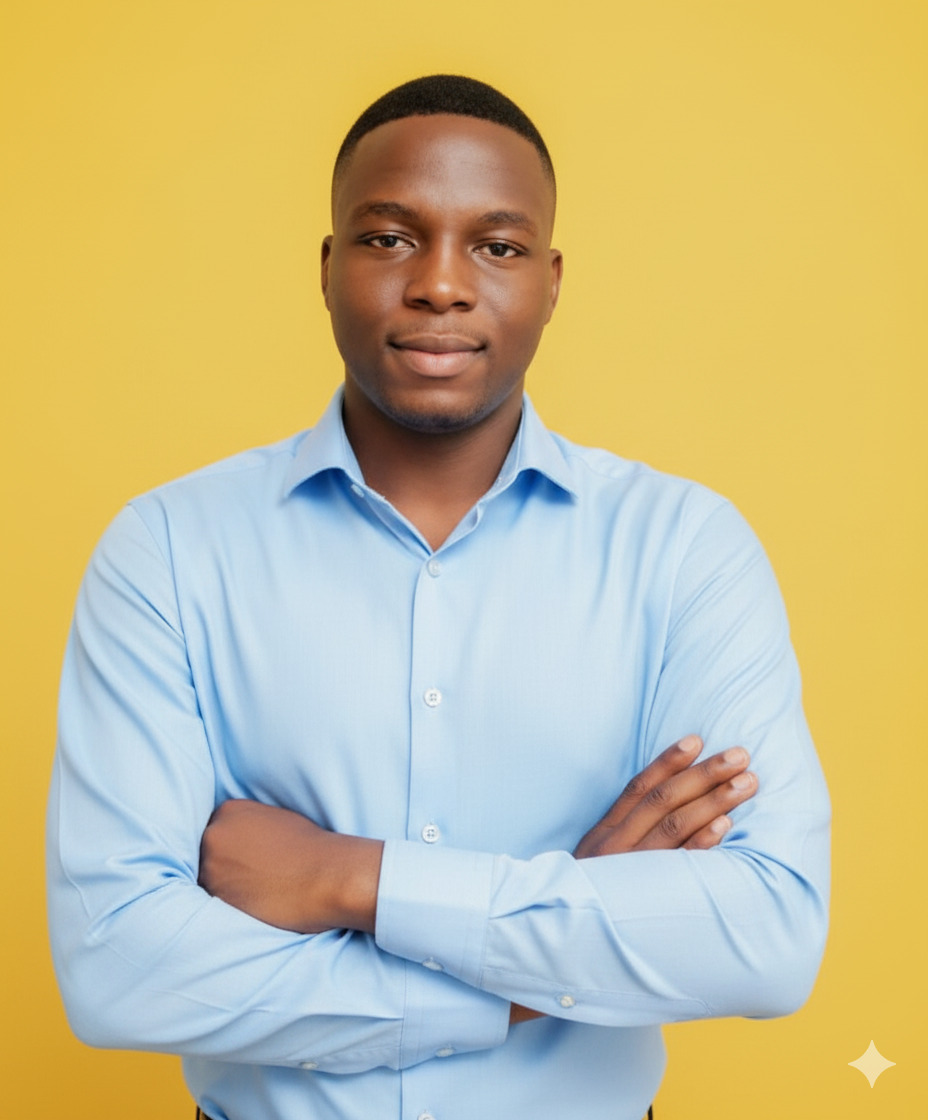
\includegraphics[width=2.9cm]{./profile.jpeg}};
    \end{scope}
    \draw[color=primary, line width=1.2pt] (0,0) circle (1.45cm);
  \end{tikzpicture}
\end{minipage}%
\hspace{0.01\textwidth}%
\begin{minipage}[c]{0.77\textwidth}
  \centering
  {\Huge \scshape \color{primary} Stéphane KPOVIESSI} \\[3pt]
  {\large \textbf{Data Scientist}} \\[7pt]
  \small
  Île-de-France (Cergy)
    \enspace$|$\enspace Disponible en CDI
    \enspace$|$\enspace +33\,7\,48\,59\,47\,13 \\[2pt]
  \href{mailto:oastephanekpoviessi@gmail.com}{oastephanekpoviessi@gmail.com}
    \enspace$|$\enspace
  \href{https://linkedin.com/in/stephanekpoviessi}{LinkedIn}
    \enspace$|$\enspace
  \href{https://github.com/EngineerProjects}{GitHub}
    \enspace$|$\enspace
  \href{https://seshat-ai.com}{Seshat-AI}
    \enspace$|$\enspace
  \href{https://kpoviessi-stephane.vercel.app/}{Portfolio}
\end{minipage}
\vspace{3pt}

\section{Profil}
\small{
Je souhaite rejoindre une équipe technique en tant que \textbf{Data Scientist junior} pour développer des solutions Data/IA utiles aux applications de l'entreprise : préparation et analyse de données, scripts Python/SQL, modèles de Machine Learning, tests et documentation. Mon expérience chez Allianz m'a permis de fiabiliser des données métiers et des traitements PySpark à grande échelle ; mes projets personnels, notamment \textbf{Seshat}, m'ont appris à intégrer des briques IA dans des applications concrètes. Je recherche un poste où progresser vite, contribuer au code et améliorer des solutions existantes avec rigueur, curiosité et esprit d'équipe.
}
\vspace{4pt}

\section{Expériences Professionnelles}
\resumeSubHeadingListStart

\resumeSubheading
{Ingénieur Data / Data Scientist}{Nov. 2025 -- Avr. 2026}
{Allianz France --- Direction P4D, Équipe Advanced Data \& Climate}{Paris, France}
\resumeItemListStart
  \resumeItem{Migration d'un datamart Assurance de SAS vers \textbf{Python/PySpark}, avec validation de la parité fonctionnelle sur plus de \textbf{15 000 lignes de code}.}
  \resumeItem{Implémentation d'une architecture \textbf{Médaillon} sur Azure Databricks intégrant plus de \textbf{150 règles métier} pour produire des datasets fiables pour l'analyse.}
  \resumeItem{Conception d'un pipeline de \textbf{Data Quality géospatiale} : contrôles de cohérence, détection d'anomalies, analyse d'écarts et sécurisation des traitements aval.}
  \resumeItem{Développement d'un framework de \textbf{tests automatisés SAS/Python} pour comparer les KPI, vérifier les seuils de tolérance et sécuriser la non-régression.}
\resumeItemListEnd

\resumeSubheading
{Data Analyst -- Missions d'appui stratégique}{2023 -- 2025}
{LYNE ET FRERES SARL \normalfont\small(Missions récurrentes d'analyse Data)}{Ikpinlè, Bénin / À distance}
\resumeItemListStart
  \resumeItem{Analyse de données commerciales, opérationnelles et de marché avec \textbf{Python/Pandas} pour suivre les KPI et identifier des leviers d'amélioration.}
  \resumeItem{Création de rapports et applications interactives avec \textbf{Streamlit} et interfaces web pour restituer les analyses aux utilisateurs métier.}
  \resumeItem{Suivi analytique des activités agricoles, notamment plantations de palmier et étapes de transformation, afin de formuler des recommandations opérationnelles.}
  \resumeItem{Accompagnement à l'usage responsable d'outils IA internes basés sur OpenWebUI et modèles open source pour appuyer les usages métier.}
\resumeItemListEnd

\resumeSubheading
{Ingénieur Machine Learning}{Mai 2024 -- Août 2024}
{Groupe Sylvagreg \normalfont\small(Stage)}{Lille, France}
\resumeItemListStart
  \resumeItem{Recherche et développement d'une solution de reconstruction 3D à partir d'images 2D, combinant Computer Vision, photogrammétrie et modèles génératifs sous \textbf{PyTorch}.}
  \resumeItem{Automatisation des pipelines de prétraitement, augmentation de données, entraînement et inférence pour fiabiliser les expérimentations.}
  \resumeItem{Déploiement cloud sur \textbf{AWS} avec conteneurisation \textbf{Docker} et interface de visualisation pour les utilisateurs métier.}
\resumeItemListEnd

\resumeSubHeadingListEnd

\section{Projet principal -- Data / IA applicative}
\resumeSubHeadingListStart

\resumeProjectHeading
{\textbf{Seshat \& Seshat-AI} $|$ \emph{Python, Go, TypeScript, Electron, React, PostgreSQL, pgvector, Chroma}}
{\href{https://github.com/EngineerProjects/seshat}{GitHub}}
\resumeItemListStart
  \resumeItem{Conception d'une plateforme Data/IA permettant d'ingérer, structurer et interroger des documents via \textbf{RAG}, recherche sémantique et bases vectorielles.}
  \resumeItem{Développement de briques applicatives en \textbf{Python}, \textbf{Go} et TypeScript, avec stockage PostgreSQL/\textbf{pgvector}, Chroma et interface desktop \textbf{Electron}/React.}
  \resumeItem{Intégration de modules IA dans une application utilisable : APIs, gestion des sessions, orchestration d'outils, tests fonctionnels, documentation et amélioration continue.}
\resumeItemListEnd

\resumeSubHeadingListEnd

\section{Autres projets sélectionnés}
\resumeSubHeadingListStart

\resumeProjectHeading
{\textbf{Solar Irradiance Forecasting} $|$ \emph{Python, Pandas, Scikit-learn, FastAPI, REST}}
{\href{https://github.com/EngineerProjects/solar-forecasting}{GitHub}}
\resumeItemListStart
  \resumeItem{Préparation et analyse de données météo : ingestion via API, nettoyage, feature engineering temporel et évaluation de modèles de prévision.}
  \resumeItem{Développement d'une \textbf{API REST FastAPI}, tests unitaires et métriques de suivi pour intégrer les prédictions dans une application exploitable.}
\resumeItemListEnd

\resumeProjectHeading
{\textbf{BI Retail Solution} $|$ \emph{Python, PySpark, Airflow, PostgreSQL, Power BI, Docker}}
{\href{https://github.com/EngineerProjects/BI_Retail}{GitHub}}
\resumeItemListStart
  \resumeItem{Chaîne data de bout en bout : ingestion, transformations \textbf{PySpark}, orchestration Airflow et chargement PostgreSQL.}
  \resumeItem{Structuration de datasets analytiques et tableaux de bord Power BI pour ventes, stocks, profits et performance logistique.}
\resumeItemListEnd

\resumeProjectHeading
{\textbf{Robot autonome de collecte de déchets} $|$ \emph{Python, YOLOv8, OpenCV, Roboflow, Dijkstra}}
{AceObject}
\resumeItemListStart
  \resumeItem{Traitement de données visuelles issues de \textbf{vidéos et images} : extraction, tri, préparation de datasets et labellisation avec \textbf{Roboflow}.}
  \resumeItem{Développement d'un pipeline Computer Vision avec \textbf{YOLOv8} et \textbf{OpenCV} pour détecter, classifier et suivre les déchets en les distinguant des obstacles.}
\resumeItemListEnd

\resumeSubHeadingListEnd

\section{Compétences}
\begin{itemize}[leftmargin=0.15in, label={}]
\small{\item{
\textbf{Analyse \& Statistiques} : Python, Pandas, NumPy, SQL, notebooks, nettoyage de données, analyse exploratoire, KPI \\
\textbf{Machine Learning} : Scikit-learn, PyTorch, TensorFlow/Keras, feature engineering, entraînement, évaluation de modèles, forecasting \\
\textbf{Data \& Big Data} : PySpark, Spark, PostgreSQL, pgvector, Chroma, Delta Lake, data quality, ETL/ELT, automatisation de traitements \\
\textbf{IA \& Applications} : RAG, LLMs, embeddings, LangGraph, LangChain, agents IA, intégration Data/IA dans applications \\
\textbf{Développement} : FastAPI, REST APIs, Go, TypeScript, React, Electron, Docker, Git, tests, documentation technique
}}
\end{itemize}

\section{Formation}
\resumeSubHeadingListStart
  \resumeSubheading
    {JUNIA ISEN}{Lille, France}
    {Diplôme d'Ingénieur --- Big Data \& Data Science}{Diplômé en 2026}
  \resumeSubheading
    {JUNIA ISEN}{Rabat, Maroc}
    {Licence --- Électronique et Systèmes Numériques}{2023}
  \resumeSubheading
    {Cycle préparatoire Marie Stella}{Cotonou, Bénin}
    {Classe préparatoire MPSI --- Mathématiques, Physique, Sciences de l'Ingénieur}{2022}
\resumeSubHeadingListEnd

\section{Langues}
\begin{itemize}[leftmargin=0.15in, label={}]
  \small{\item{
   \textbf{Français} : Langue maternelle \vspace{1.5pt} \\
   \textbf{Anglais} : B2 | Linguaskill Business English \vspace{1.5pt} \\
   \textbf{Yoruba, Fon, Goun} : Langues maternelles (Bilingue)
  }}
\end{itemize}

\section{Certifications}
\begin{itemize}[leftmargin=0.15in, label={}]
\small{\item{
\textbf{Supervised Machine Learning} | \href{https://www.coursera.org/learn/machine-learning}{DeepLearning.AI} $|$ 2023 \vspace{1.5pt} \\
\textbf{Data Analysis with Python} | freeCodeCamp $|$ 2023 \vspace{1.5pt} \\
\textbf{Create Machine Learning Models in Microsoft Azure} | Microsoft $|$ 2023
}}
\end{itemize}

\section{Engagements \& Associations}
\resumeSubHeadingListStart
  \resumeSubheading
    {Vice-Président | Commission Réseau JUNIA ALUMNI}{Sep. 2024 -- Août 2025}
    {Coordination du réseau, engagement des alumni et organisation d'événements professionnels}{Lille, France}

  \resumeSubheading
    {Responsable Communication | Commission Réseau JUNIA ALUMNI}{Sep. 2023 -- Août 2024}
    {Communication et promotion des initiatives alumni}{Lille, France}
\resumeSubHeadingListEnd

\end{document}
